\begin{appendix}



\chapter{Chapter and Section authors}

\section{Dominik Horb}
Introduction \\
Chapter Project Overview \\
Chapter Project Analysis and Outlook

\section{Elsa Mahari}
Chapter Features -- User avatar – introduction part\\
Chapter Features -- Report\\
Chapter Project Analysis and Outlook -- summaryAndOutlook -- Project Analysis -- communication part

\section{Tien Nguyen}
Chapter Features -- Simtext\\
Chapter Features -- BibTex

\section{Benjamin Oertel}
Chapter Features -- Notifications and Comments\\
Chapter Features -- Fragments\\
Chapter Features -- User avatar – cropping mechanism part \\
Chapter Features -- Automatic Plagiarism Detection Webservices \\
Chapter Features -- Permission and role management \\
Chapter Features -- Barcode

\section{Heiko Stammel:}
Chapter Showtime \\


\chapter{Logged Time}

In the following we try to display the time that was logged on the project between 1st of April and 26th of July 2012 according to our Redmine system. Please keep in mind that this information may not be totally accurate.

At first you can see the overview of all the members and the logged hours.

% should be updated later on, now simply to make sure it works
% generate various reports in redmine and export as csv
% don't forget to escape special characters like _ or # in the input .csv, e. g. \_ or \#

\DTLloaddb{overview}{data/timelog-overview.csv}
\begin{table}[htbp]
  \caption{Overview By Member and Month}
  \centering
  \DTLdisplaydb{overview}
\end{table}

The next sections show all single entries per team member. Mostly the times were logged regarding one ticket in the system, but some small blocks were sometimes also logged without creating a ticket.

\begin{landscape}
\section{Time by Elsa Mahari}
\DTLloaddb{elsa}{data/elsa.csv}
\DTLdisplaylongdb[caption=Time logged for tickets]{elsa}
\end{landscape}

\begin{landscape}
\section{Time by Tien Nguyen}
\DTLloaddb{tien}{data/tien.csv}
\DTLdisplaylongdb[caption=Time logged for tickets]{tien}
\end{landscape}

\begin{landscape}
\section{Time by Heiko Stammel}
\DTLloaddb{heiko}{data/heiko.csv}
\DTLdisplaylongdb[caption=Time logged for tickets]{heiko}
\end{landscape}

\begin{landscape}
\section{Time by Dominik Horb}
\DTLloaddb{dominik}{data/dominik.csv}
\DTLdisplaylongdb[caption=Time logged for tickets]{dominik}

\DTLloaddb{dominikNoTicket}{data/dominik-no-ticket.csv}
\DTLdisplaylongdb[caption=Time logged without tickets]{dominikNoTicket}

\end{landscape}

% \begin{landscape}

% \DTLsetseparator{,}

% \DTLloaddb{issueMember}{data/timelog-issue-member.csv}
%   \centering
%  \DTLdisplaylongdb[caption=Overview By Member and Issue]{issueMember}

% \DTLloaddb{sprints}{data/timelog-sprints.csv}
% \begin{table}[htbp]
%   \caption{Overview By Sprints}
%   \centering
%   \DTLdisplaydb{sprints}
% \end{table}

% \end{landscape}

\includepdf[pages=1-3]{data/timelog_benjamin.pdf}


\chapter{Showtime}

\begin{figure}[!h]
  \centering
    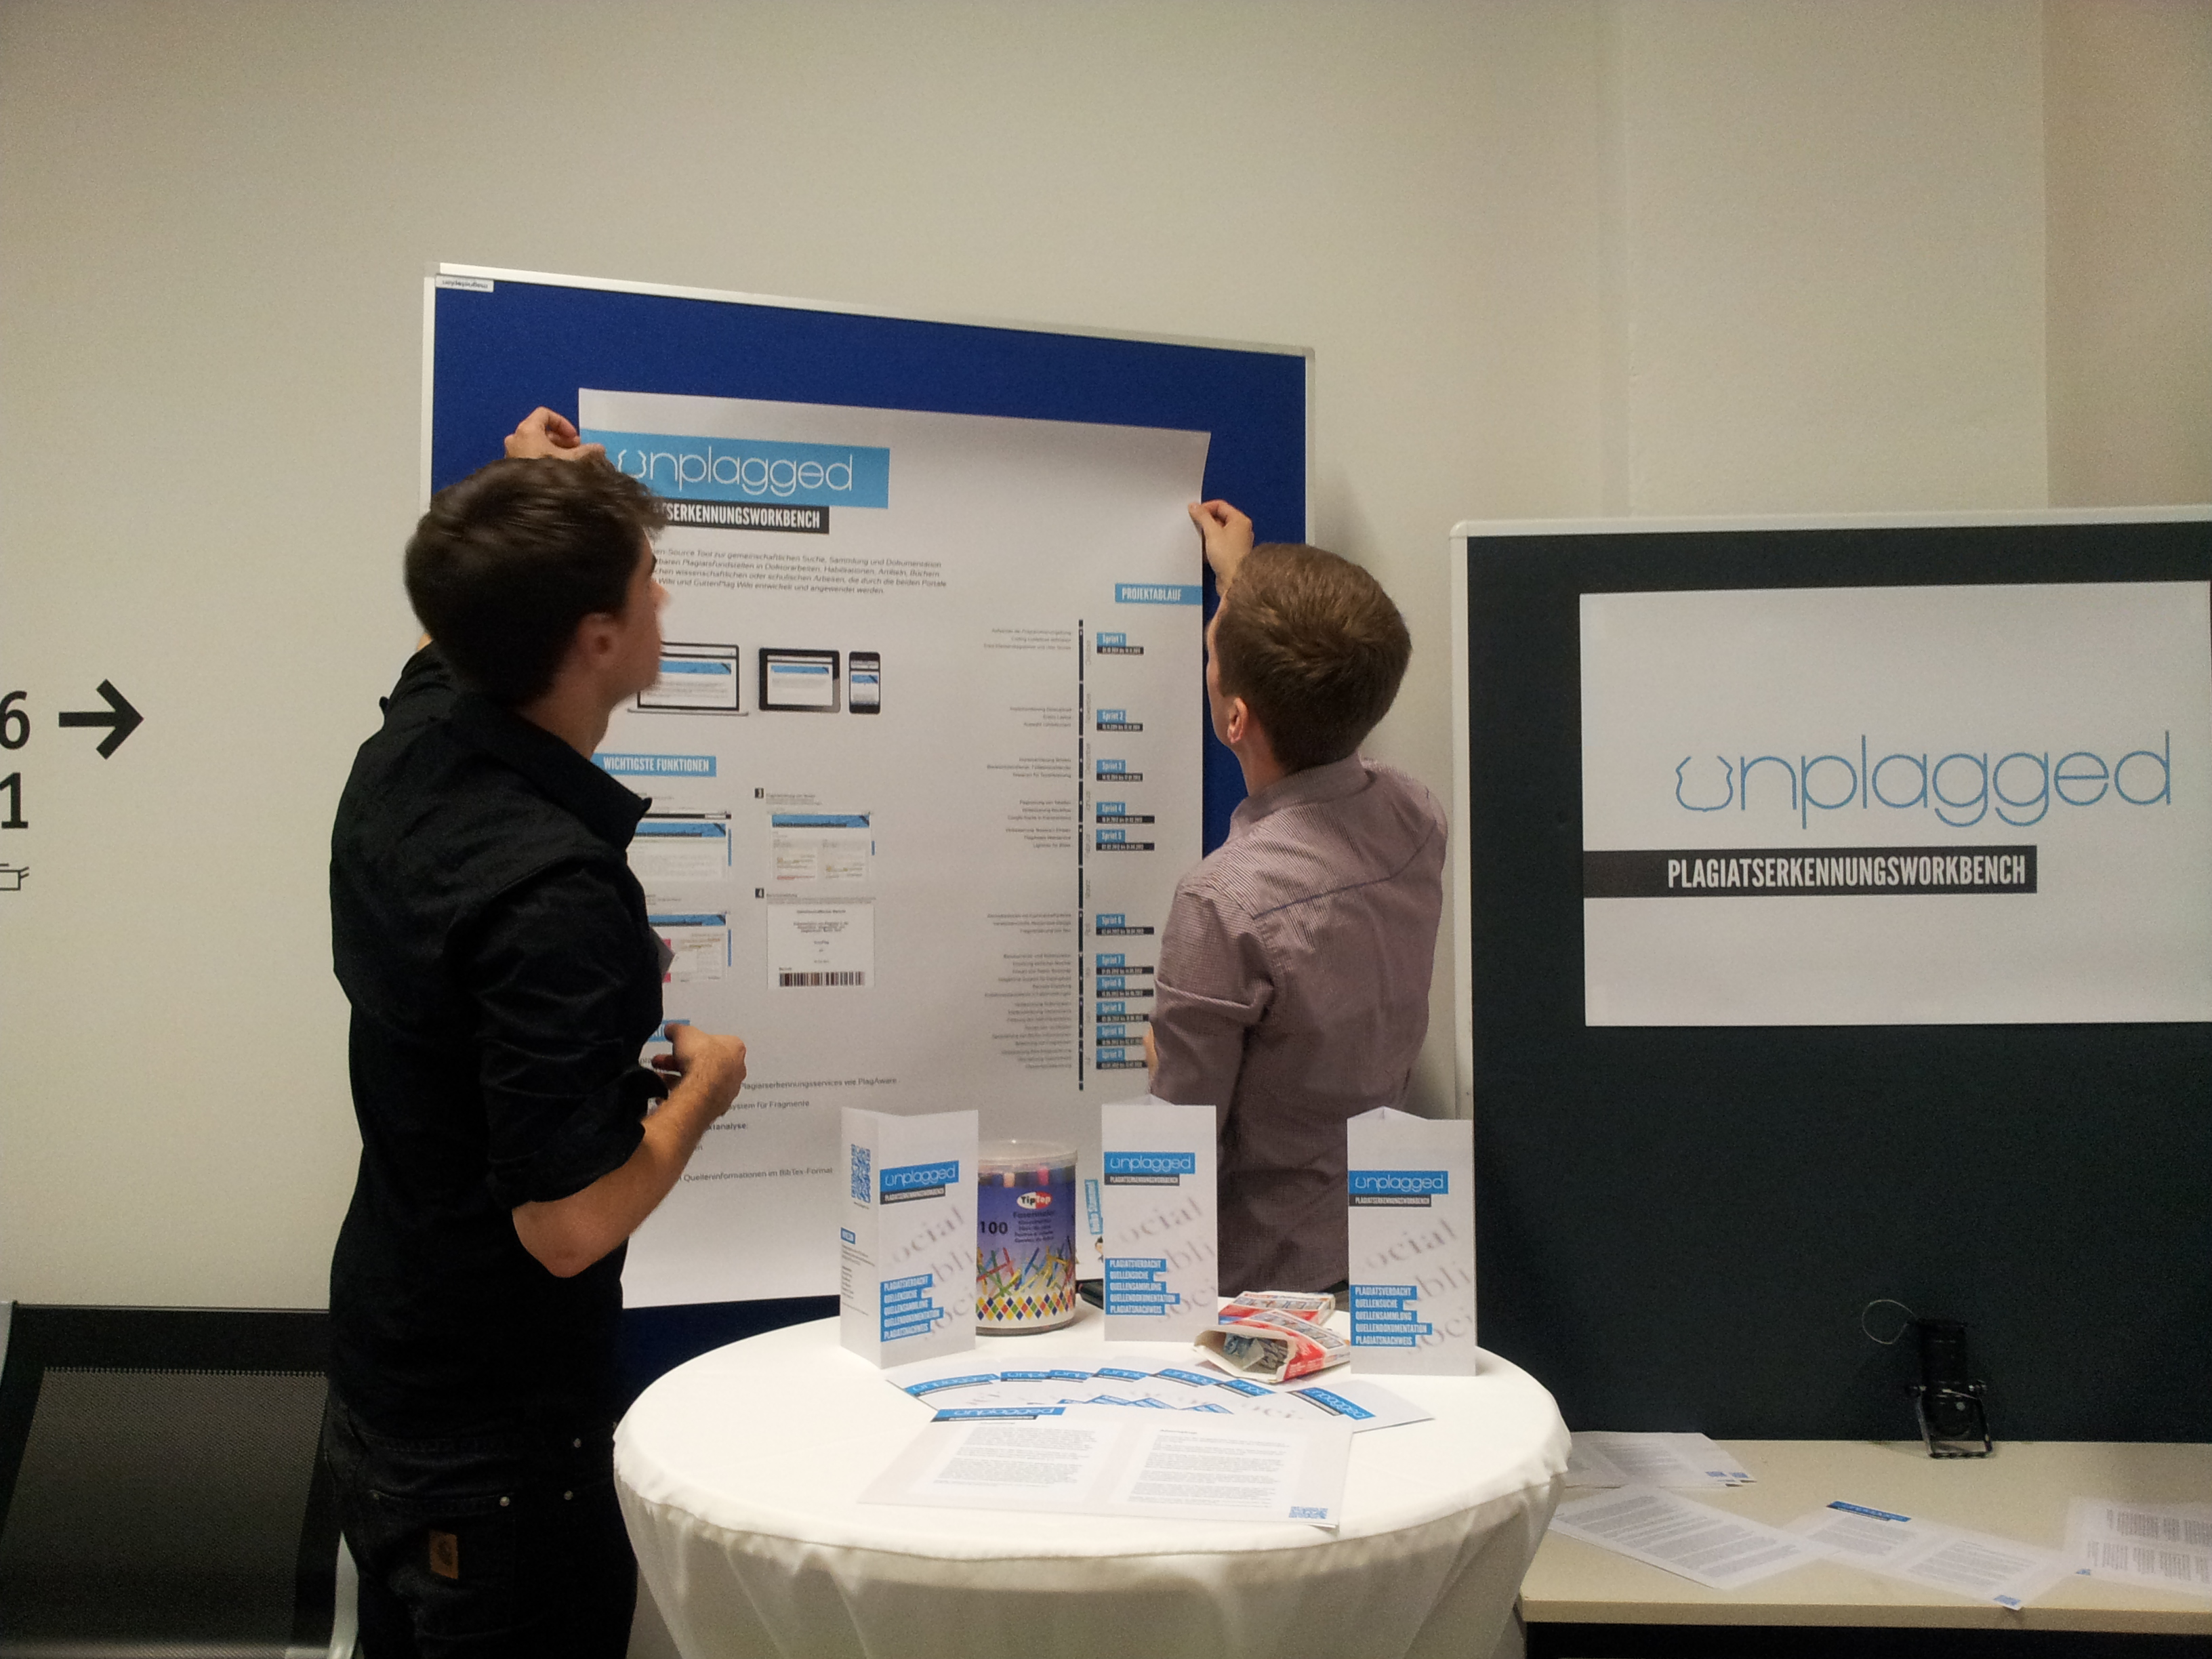
\includegraphics[width=0.97\textwidth]{images/unplagged_exhibition_stand1.jpg}
  \caption{Unplagged's exhibition stand}
  \label{fig:unplagged_exhibition_stand1}
\end{figure}

\begin{figure}[!h]
  \centering
    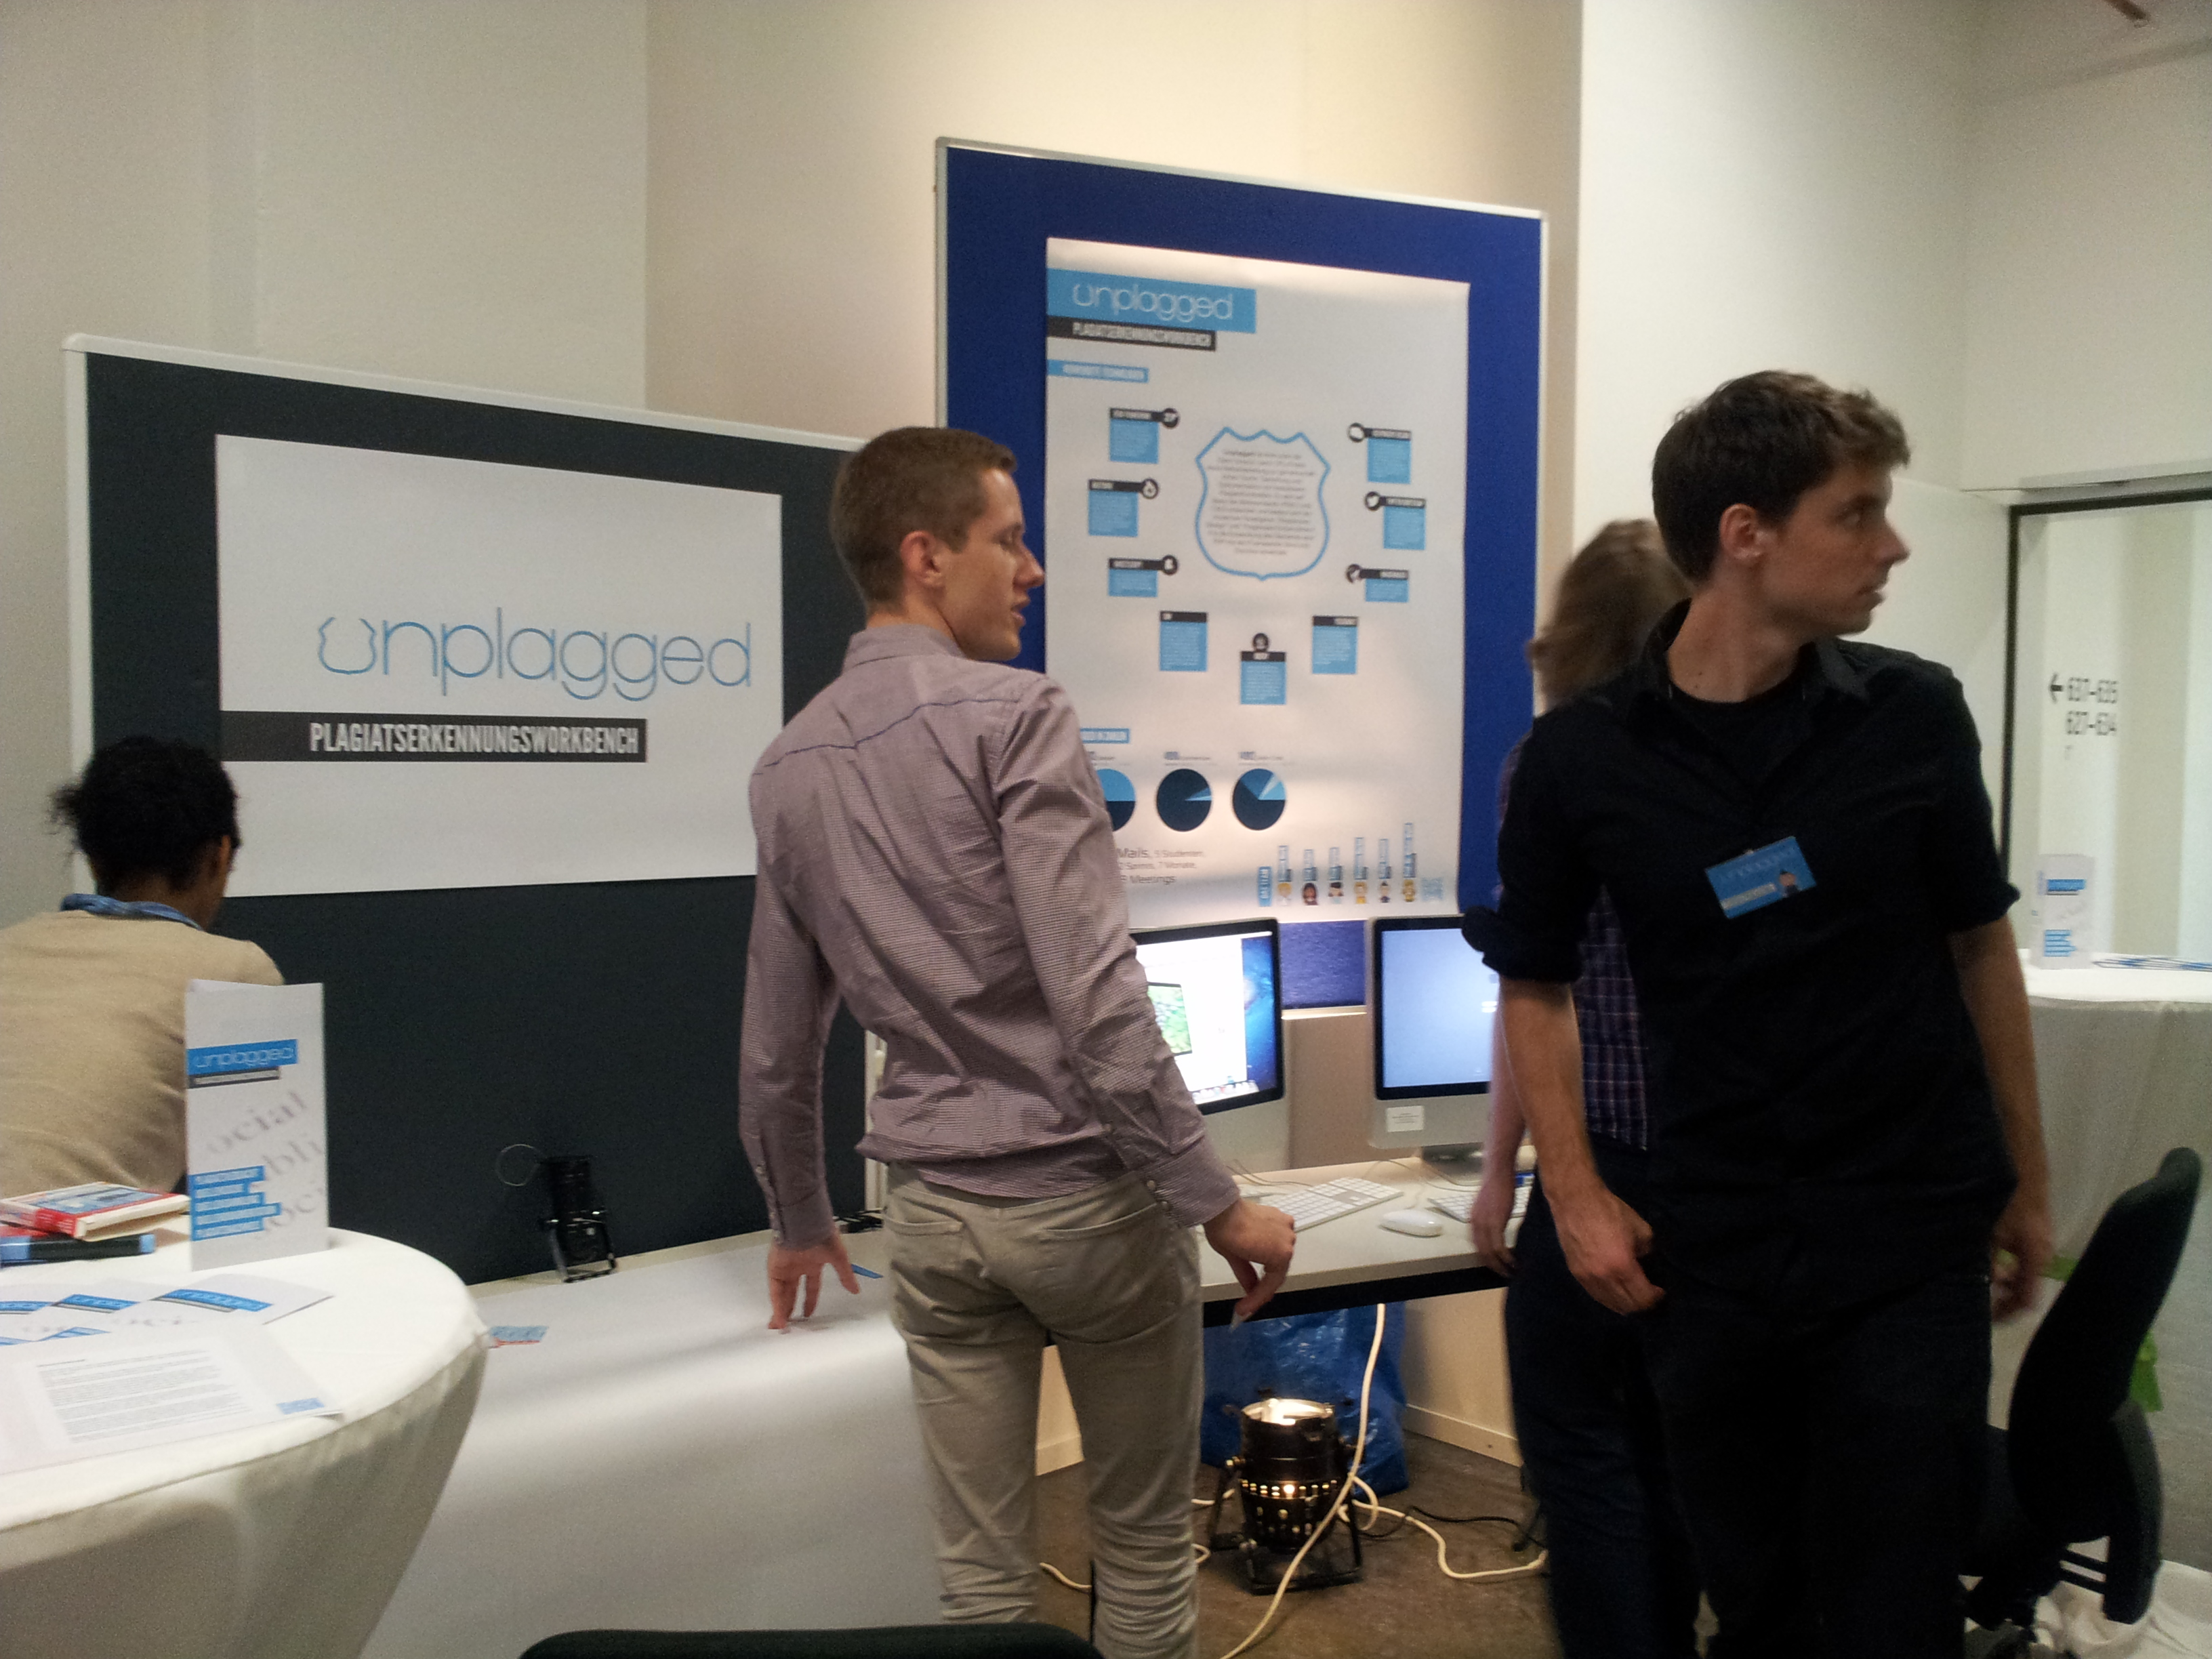
\includegraphics[width=0.97\textwidth]{images/unplagged_exhibition_stand2.jpg}
  \caption{Unplagged's exhibition stand}
  \label{fig:unplagged_exhibition_stand2}
\end{figure}

\begin{figure}[!h]
  \centering
    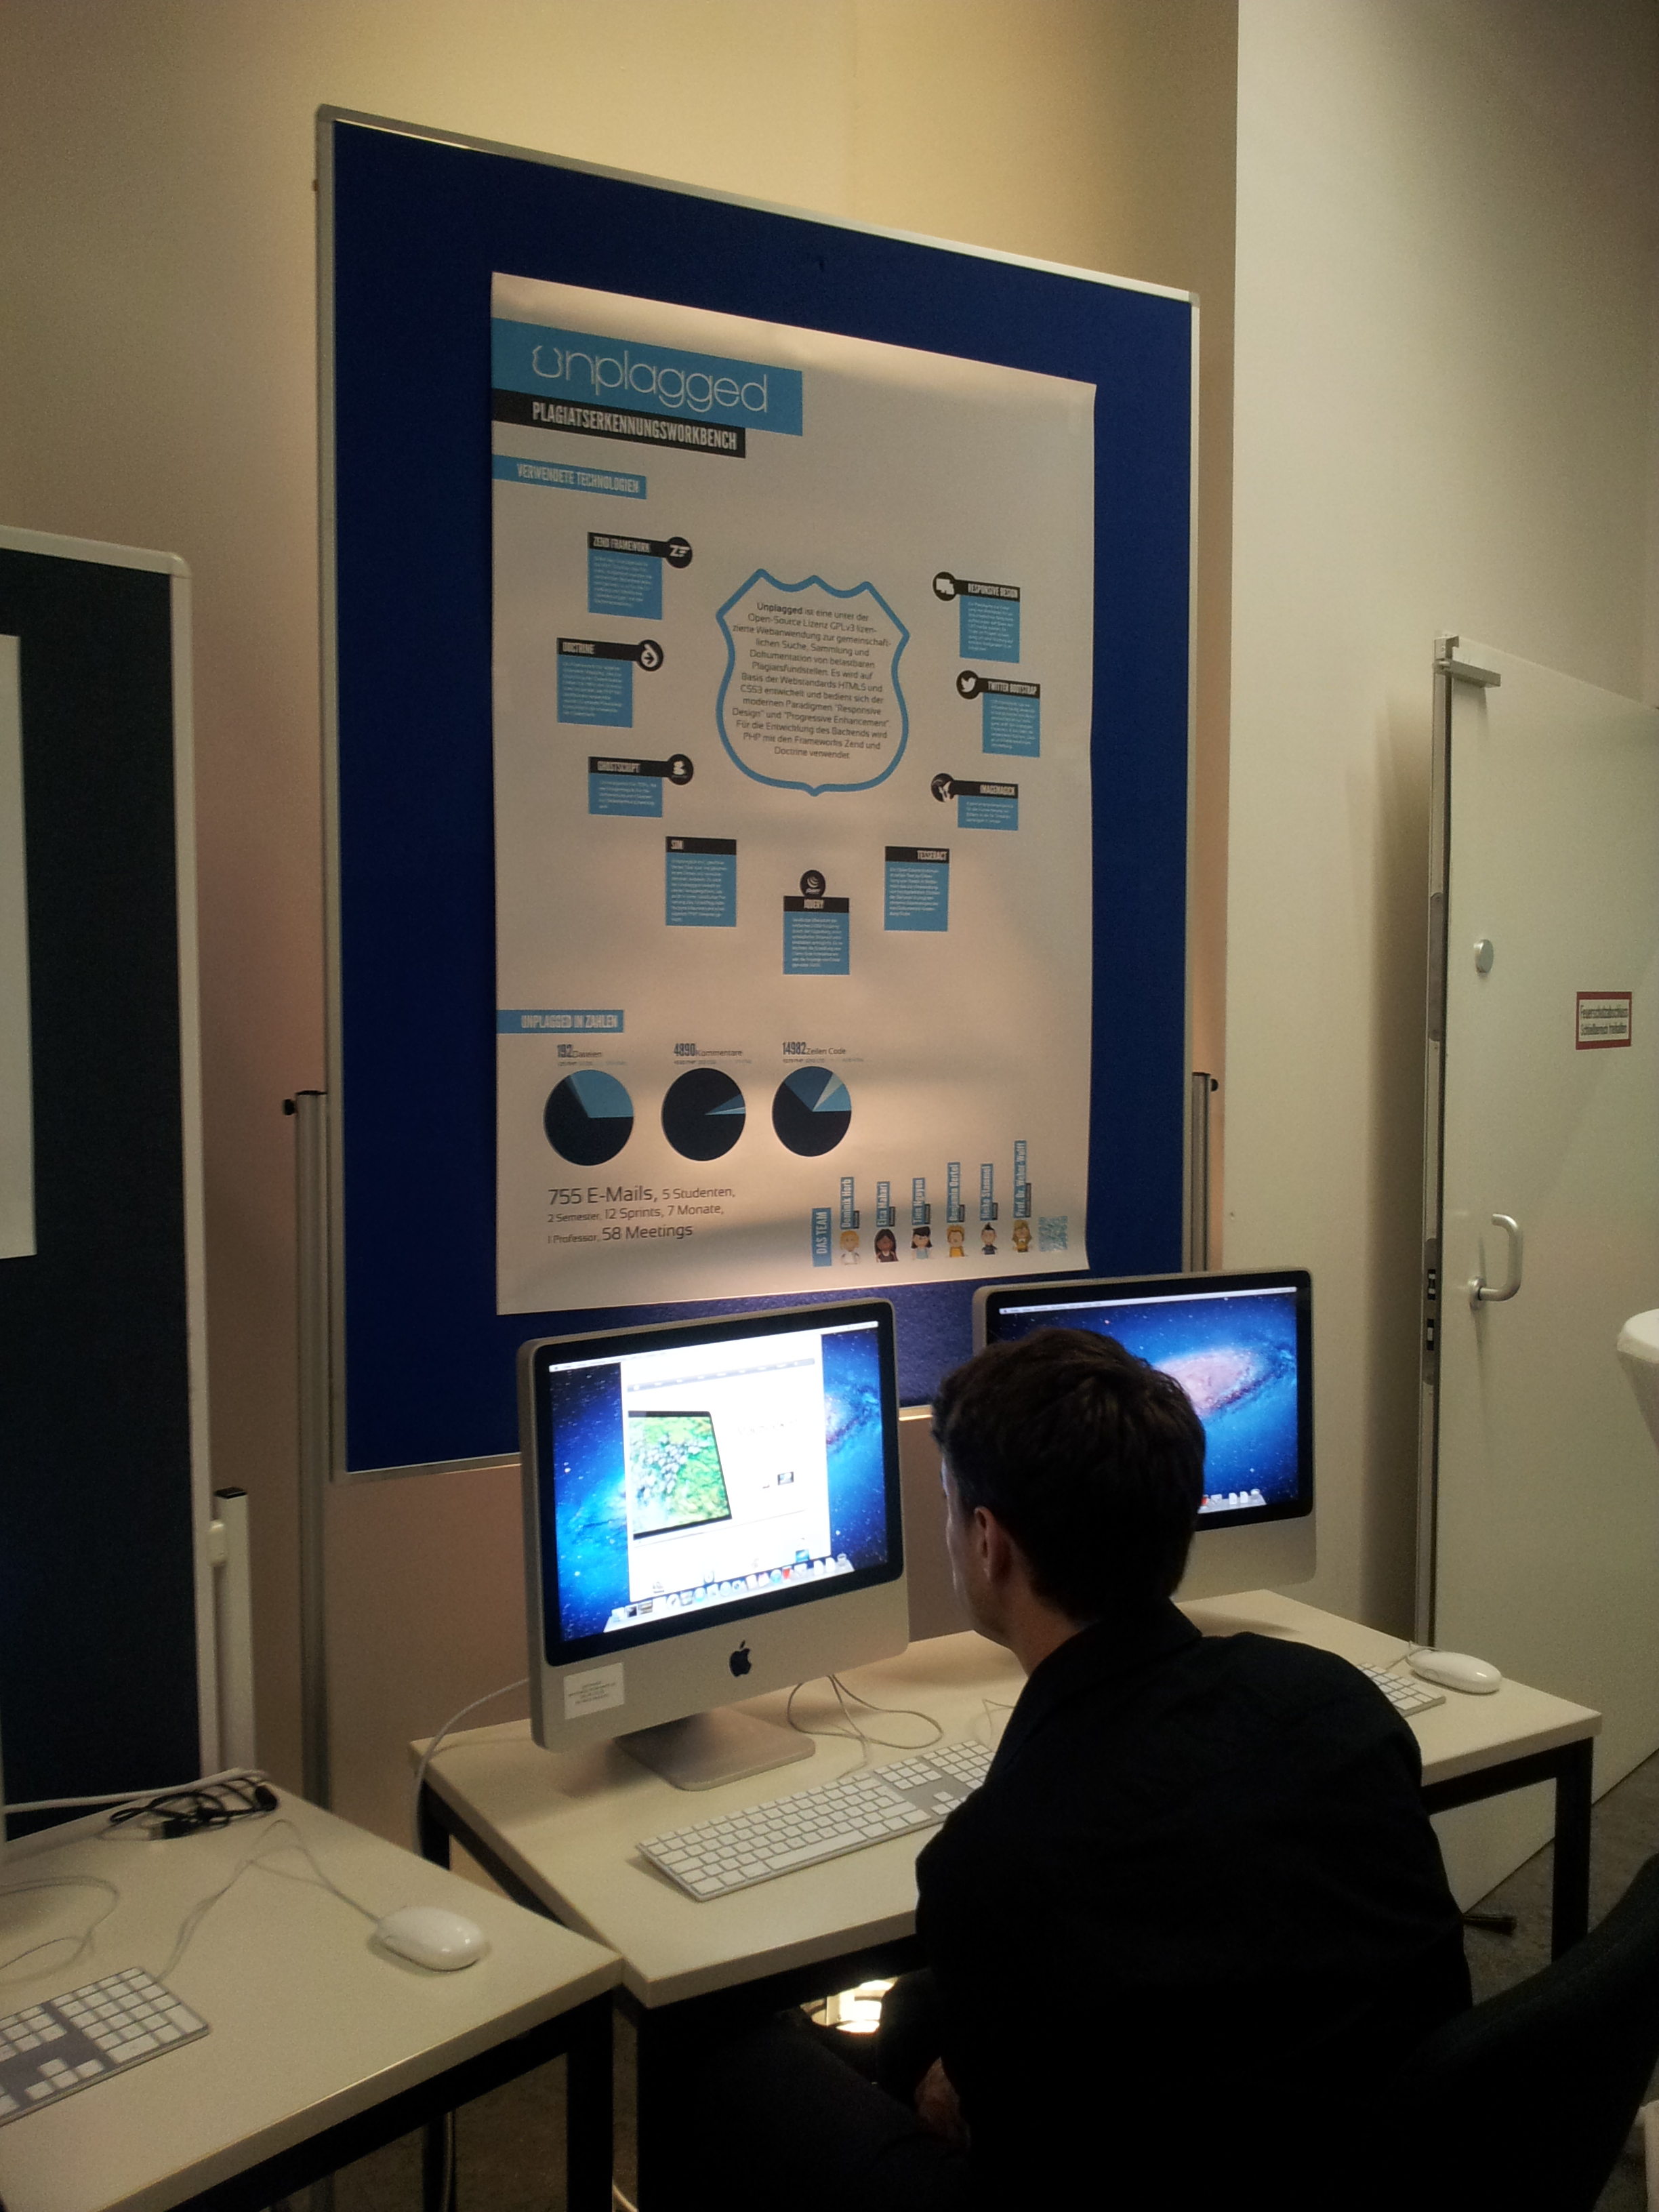
\includegraphics[width=0.97\textwidth]{images/unplagged_exhibition_stand3.jpg}
  \caption{Unplagged's exhibition stand}
  \label{fig:unplagged_exhibition_stand3}
\end{figure}

\begin{figure}[!h]
  \centering
    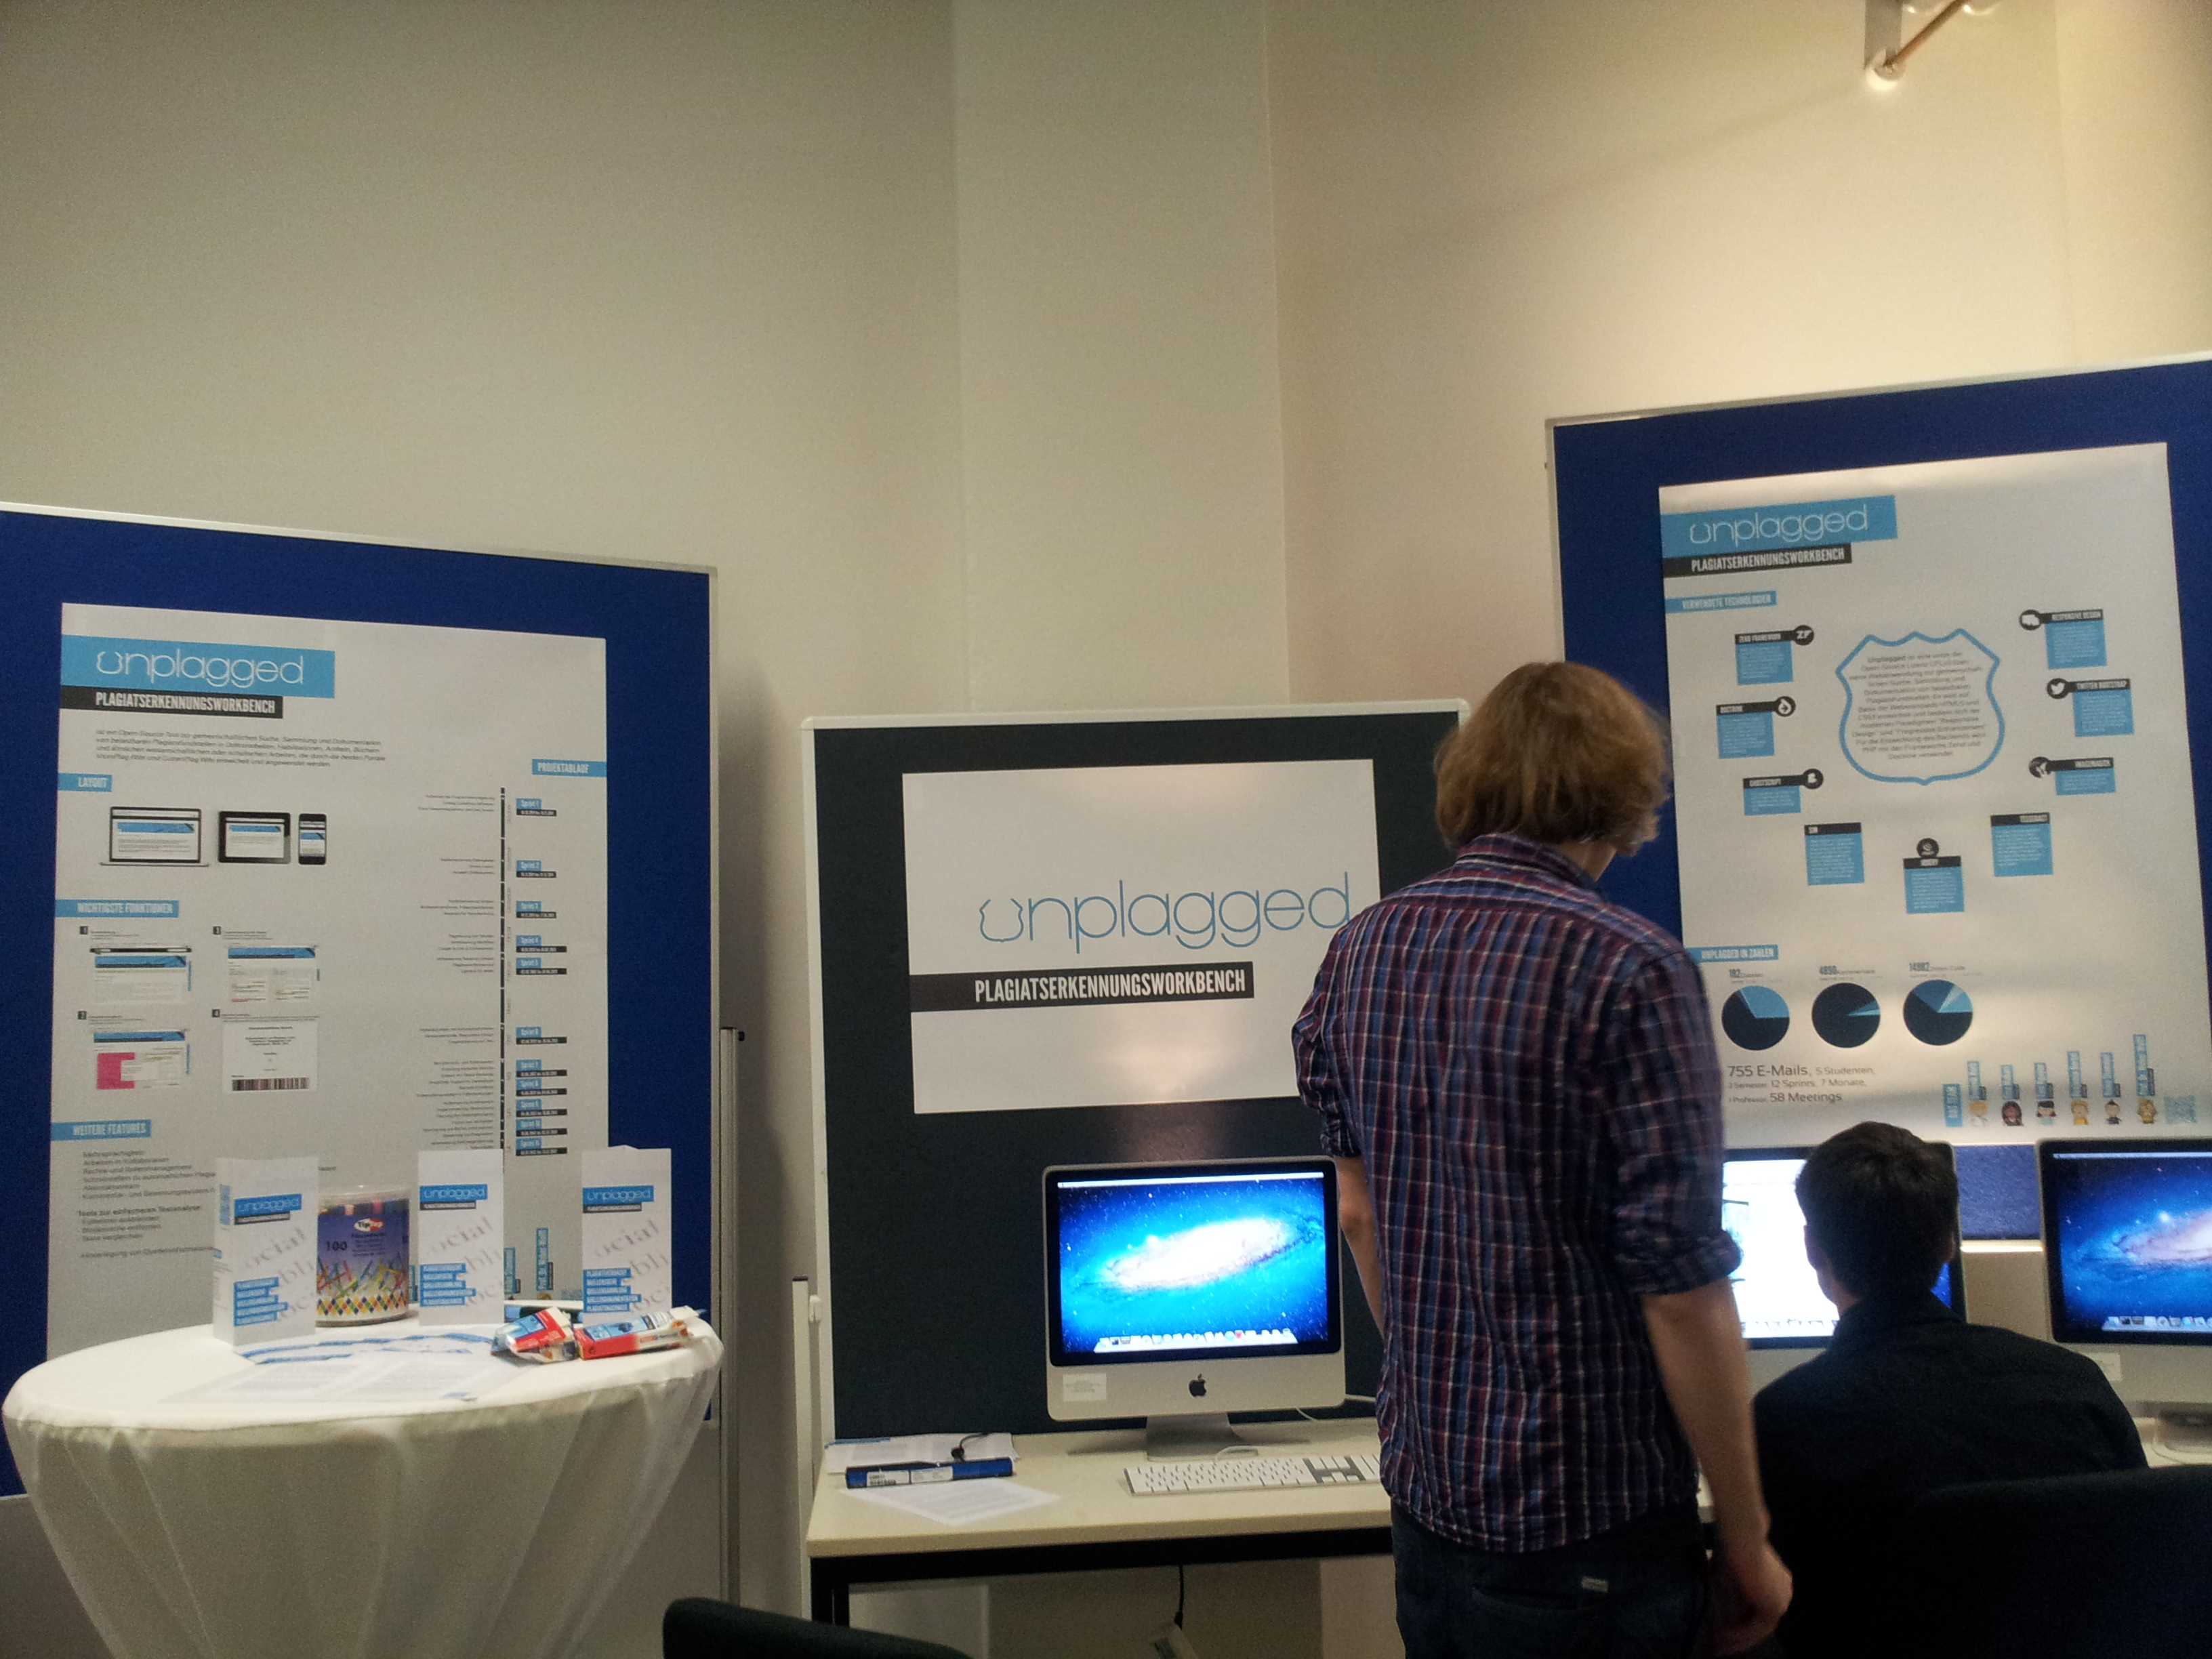
\includegraphics[width=0.97\textwidth]{images/unplagged_exhibition_stand4.jpg}
  \caption{Unplagged's exhibition stand}
  \label{fig:unplagged_exhibition_stand4}
\end{figure}

\end{appendix}
